\documentclass{hitec}
\newcommand{\HT}{\textsc{\raisebox{0.1em}{h}\raisebox{-0.1em}{i}%
		\raisebox{0.1em}{t}\raisebox{-0.1em}{e}\raisebox{0.1em}{c} }}


% set shortcuts
%% Package, Library, abbreviate terms
\newcommand{\siplibtwo}{\textsf{SIPLIB 2.0}}
\newcommand{\siplib}{\textsf{SIPLIB}}
\newcommand{\miplib}{\textsf{MIPLIB 2010}}
\newcommand{\smps}{\textsf{SMPS}}
\newcommand{\mps}{\textsf{MPS}}
\newcommand{\mpsx}{\textsf{MPSX}}
\newcommand{\jump}{\textsf{JuMP}}
\newcommand{\structjump}{\textsf{StructJuMP}}

% Problems
\newcommand{\dcap}{\textsf{DCAP}}
\newcommand{\dclp}{\textsf{DCLP}}
\newcommand{\mptsps}{\textsf{MPTSPs}}
\newcommand{\sizes}{\textsf{SIZES}}
\newcommand{\smkp}{\textsf{SMKP}}
\newcommand{\sslp}{\textsf{SSLP}}
\newcommand{\suc}{\textsf{SUC}}

% Solvers
\newcommand{\dsp}{\textsf{DSP}}
\newcommand{\pysp}{\textsf{PySP}}
\newcommand{\pyomo}{\textsf{Pyomo}}
\newcommand{\cplex}{\textsf{CPLEX}}

%% Programming languages
\newcommand{\julia}{\texttt{Julia}}
\newcommand{\python}{\texttt{Python}}
\newcommand{\clang}{\texttt{C}}
\newcommand{\cpp}{\texttt{C++}}
\newcommand{\matlab}{\texttt{MATLAB}}

%% Siplib.jl related terms
\newcommand{\jumpmodel}{\texttt{JuMP.Model}}
\newcommand{\siplibjl}{\texttt{Siplib.jl}}

\newcommand{\kk}[1]{{\color{blue}From Kibaek: #1}}
\newcommand{\yoc}[1]{{\color{NavyBlue}From Yongkyu: #1}}
\newcommand{\stkout}[1]{\ifmmode\text{\sout{\ensuremath{#1}}}\else\sout{#1}\fi}

\title{\siplibjl: A \julia\ package for \siplibtwo}
\author{Yongkyu Cho}
\company{IME, POSTECH}
\confidential{\textbf{-- Prototype Manual --}}

\usepackage{hyperref}
\usepackage[usenames,dvipsnames]{xcolor}
\usepackage{graphicx}
\usepackage{hyperref}
\usepackage{mathrsfs,amsmath,amssymb,amscd,mathtools}
\usepackage{booktabs}
\usepackage{graphicx}
\usepackage{lscape}
\usepackage{color}
\usepackage{multirow}
\usepackage{booktabs}
\usepackage{subfig}
\usepackage{float}
\usepackage{caption}
\usepackage{filecontents}
\usepackage[normalem]{ulem}
\usepackage[flushleft]{threeparttable}
\usepackage{stfloats}
\usepackage{lscape}
\usepackage{longtable}
\usepackage{listings}
\usepackage{courier}
\usepackage{soul}
\usepackage{forest}
\usepackage[graphicx]{realboxes}

\definecolor{folderbg}{RGB}{124,166,198}
\definecolor{folderborder}{RGB}{110,144,169}

\def\Size{4pt}
\tikzset{
	folder/.pic={
		\filldraw[draw=folderborder,top color=folderbg!50,bottom color=folderbg]
		(-1.05*\Size,0.2\Size+5pt) rectangle ++(.75*\Size,-0.2\Size-5pt);  
		\filldraw[draw=folderborder,top color=folderbg!50,bottom color=folderbg]
		(-1.15*\Size,-\Size) rectangle (1.15*\Size,\Size);
	}
}

\lstdefinelanguage{julia}
{
	sensitive=true,	
	basicstyle=\ttfamily\scriptsize,
	columns=fullflexible, % make sure to use fixed-width font, CM typewriter is NOT fixed width
	numbers=left, 
	numberstyle=\small\ttfamily\color{Gray},
	stepnumber=0,              
	numbersep=10pt, 
	numberfirstline=true, 
	numberblanklines=true, 
	tabsize=4,
	lineskip=-1.5pt,
	extendedchars=true,
	breaklines=true,        
	keywordstyle=\color{Blue}\bfseries,
	identifierstyle=, % using emph or index keywords
	commentstyle=\sffamily\color{OliveGreen},
	stringstyle=\color{Maroon},
	showstringspaces=false,
	showtabs=false,
	upquote=false,
	keywordsprefix=\@,
	keywords={exit,whos,edit,load,is,isa,isequal,typeof,tuple,ntuple,uid,hash,finalizer,convert,promote,
		subtype,typemin,typemax,realmin,realmax,sizeof,eps,promote_type,method_exists,applicable,
		invoke,dlopen,dlsym,system,error,throw,assert,new,Inf,Nan,pi,im,begin,while,for,in,return,
		break,continue,macro,quote,let,if,elseif,else,try,catch,end,bitstype,ccall,do,using,module,
		import,export,importall,baremodule,immutable,local,global,const,Bool,Int,Int8,Int16,Int32,
		Int64,Uint,Uint8,Uint16,Uint32,Uint64,Float32,Float64,Complex64,Complex128,String,Symbol,Any,Nothing,None,
		function,type,typealias,abstract,struct, mutable},
	comment=[l]{\#},
	%morecomment=[s]{#=}{=#},
	morestring=[d]\',
	morestring=[b]\",
}


\graphicspath{{./figures/}}

% set table of contents depths
\setcounter{tocdepth}{2}

\DeclareMathOperator*{\PP}{\mathbb{P}}
\DeclareMathOperator*{\EE}{\mathbb{E}}
\DeclarePairedDelimiter\ceil{\lceil}{\rceil}
\DeclarePairedDelimiter\floor{\lfloor}{\rfloor}

\begin{document}
	\maketitle
	\section{Introduction}
	\siplibtwo\ is an extended version of \siplib, the first SIP-oriented instance collection constructed in 2002 by Shabbir Ahmed and his colleagues \cite{web:SIPLIB1}. We implement a \julia\ package for users to utilize new funtionalities of \siplibtwo. 
	
	In this manual, we introduce the package. The main functionality of \siplibjl\ is to generate \smps\ files of instances of stochastic integer programming (SIP) problems. Currently supported problems and corresponding instance names are summarized in Table \ref{table:problems} and Table \ref{table:naming_rule}.
%	\begin{table}[H]
%		\centering
%		\resizebox{\textwidth}{!}{%
%			\begin{threeparttable}
%				\caption{Problems in \siplibtwo}
%				\label{table:problems}
%				\begin{tabular}{@{}llll@{}}
%					\toprule
%					Problem		  		  & Description                                                        & Main reference              \\ \midrule
%					\dcap\         & Dynamic capacity planning with stochastic demand (\ref{DCAP})                   & Ahmed and Garcia \cite{journal:AG2004}                          \\
%					\mptsps\       & Multi-path traveling salesman problem with stochastic travel costs (\ref{MPTSPs})& Tadei et al. \cite{journal:TPP2017}                            \\
%					\sizes\        & Optimal product substitution with stochastic demand (\ref{SIZES})         & Jorjani et al. \cite{journal:JSW1999}          \\
%					\smkp\		  & Stochastic multiple knapsack problem (\ref{SMKP})                              & Angulo et al. \cite{journal:AAD2014}                            \\
%					\sslp\         & Stochastic server location problem (\ref{SSLP})                                & Ntaimo and Sen \cite{journal:NS2005}                           \\
%					\suc\         & Stochastic unit commitment problem	(\ref{SUC})			               & Papavasiliou and Oren \cite{journal:PO2013}                       \\ \bottomrule
%				\end{tabular}%
%				
%				%			\begin{tablenotes}
%				%				\small
%				%				\item For convenience, we skip the cardinality sign $|\cdot|$ for sets, i.e., for any set $S$, $S$ denotes the number of elements $|S|$ in this table.
%				%			\end{tablenotes}
%			\end{threeparttable}
%		}
%	\end{table}

	\begin{table}[H]
	\centering
	\resizebox{\textwidth}{!}{%
		\begin{threeparttable}
			\caption{Problems in \siplibtwo}
			\label{table:problems}
			\begin{tabular}{@{}llll@{}}
				\toprule
				Problem		  		  & Description                                                        & Main reference              \\ \midrule
				\dcap\         & Dynamic capacity planning with stochastic demand                   & Ahmed and Garcia \cite{journal:AG2004}                          \\
				\mptsps\       & Multi-path traveling salesman problem with stochastic travel costs & Tadei et al. \cite{journal:TPP2017}                            \\
				\sizes\        & Optimal product substitution with stochastic demand          & Jorjani et al. \cite{journal:JSW1999}          \\
				\smkp\		  & Stochastic multiple knapsack problem                               & Angulo et al. \cite{journal:AAD2014}                            \\
				\sslp\         & Stochastic server location problem                                 & Ntaimo and Sen \cite{journal:NS2005}                           \\
				\suc\         & Stochastic unit commitment problem			               & Papavasiliou and Oren \cite{journal:PO2013}                       \\ \bottomrule
			\end{tabular}%
			
			%			\begin{tablenotes}
			%				\small
			%				\item For convenience, we skip the cardinality sign $|\cdot|$ for sets, i.e., for any set $S$, $S$ denotes the number of elements $|S|$ in this table.
			%			\end{tablenotes}
		\end{threeparttable}
		}
	\end{table}
	
	\begin{table}[]
		\centering
		\caption{Instance naming rules}
		\label{table:naming_rule}
		\resizebox{\textwidth}{!}{%
			\begin{tabular}{@{}lll@{}}
				\toprule
				Problem & Instance name                 & Remark                                                                    					      \\ \midrule
				\dcap\    & DCAP\_$R$\_$N$\_$T$\_$\mathcal{S}$    &   $R$: number of resources, $N$: number of tasks, $T$: number of time periods, $\mathcal{S}$: number of scenarios        \\
				\mptsps\  & MPTSPs\_$D$\_$N$\_$\mathcal{S}$ &$D$: node distribution strategy, $N$: number of nodes, $\mathcal{S}$: number of scenarios\\
				\sizes\   & SIZES\_$\mathcal{S}$                            & $\mathcal{S}$: number of scenarios   															\\
				\smkp\    &   SMKP\_$I$\_$\mathcal{S}$    &   $I$:number of types for item, $\mathcal{S}$: number of scenarios  													 \\
				\sslp\    &  SSLP\_$I$\_$J$\_$\mathcal{S}$      &    $I$: number of clients, $J$: number of server locations, $\mathcal{S}$: number of scenarios                 				   \\
				\suc\    & 	SUC\_$D$\_$\mathcal{S}$    &  $D$: day type, $\mathcal{S}$: number of scenarios                                                 						 \\ \bottomrule
			\end{tabular}%
		}
	\end{table}

	\subsection{Preliminaries}
	\subsubsection{\smps\ format} \label{subsec:smps}
	\smps\ format is a data conventions for the automatic input of multiperiod stochastic linear programs. The input format is based on an old column-oriented format \mpsx\ standard and is designed to promote the efficient conversion of originally deterministic problems by introducing stochastic variants in separate files. 
	
	Three input files are required to specify an stochastic program (SP) in \smps\ format:
	\begin{itemize}
		\item \texttt{.cor}: Core file written in \mps\ format. This describes the fundamental problem structure and contains the first-stage data and one second-stage scenario data.
		\item \texttt{.tim}: Time file which specifies the location where the second-stage begins.
		\item \texttt{.sto}: Stoch file which contains stochastic data of all scenarios except the one included in \texttt{.cor} file.
	\end{itemize}
	One of the main functions of the package is to generate \smps\ files for an instance. For example, the package generates the following three files for a \dcap\ instance \dcap\_$R$\_$N$\_$T$\_$S$.
	\begin{itemize}
		\item \texttt{DCAP\_R\_N\_T\_S.cor}
		\item \texttt{DCAP\_R\_N\_T\_S.tim}
		\item \texttt{DCAP\_R\_N\_T\_S.sto}
	\end{itemize}
	%\kk{This needs moved to later section.} \yoc{I move this to this section.}
	
	\subsubsection{\jumpmodel-type object}
	\jumpmodel-type object is an object that contains every information of an instance. Hence, almost every function in the package requires this object as one of its input arguments. Combining \structjump\ package together with \jump\ package, constructing a \jumpmodel\ object is quite simpler and more intuitive than any other algebraic modeling language dedicated for SIP. For example, the script in Fig. \ref{fig:dcap_models} constructs an object \texttt{model} of a \dcap\_$R$\_$N$\_$T$\_$S$ instance.
	
	\subsection{Structure of the \julia\ package}
	The tree in Fig. \ref{fig:siplibjl_structure} shows how the \julia\ package is structured. 
	\begin{figure}[H] 
		\centering   
		\begin{forest}
			for tree={
				font=\ttfamily,
				grow'=0,
				child anchor=west,
				parent anchor=south,
				anchor=west,
				calign=first,
				inner xsep=7pt,
				edge path={
					\noexpand\path [draw, \forestoption{edge}]
					(!u.south west) +(7.5pt,0) |- (.child anchor) pic {folder} \forestoption{edge label};
				},
				% style for your file node 
				file/.style={edge path={\noexpand\path [draw, \forestoption{edge}]
						(!u.south west) +(7.5pt,0) |- (.child anchor) \forestoption{edge label};},
					inner xsep=2pt,font=\small\ttfamily
				},
				before typesetting nodes={
					if n=1
					{insert before={[,phantom]}}
					{}
				},
				fit=band,
				before computing xy={l=15pt},
			}  
			[Siplib
			[src
			[problems
			[DCAP
			[dcap\_types.jl,file]
			[dcap\_functions.jl,file]
			[dcap\_models.jl,file]
			]
			[MPTSPs]
			[SIZES
			[DATA
			[oneperioddata.csv,file]
			]
			[sizes\_types.jl,file]
			[sizes\_functions.jl,file]
			[sizes\_models.jl,file]			
			]
			[SMKP]
			[SSLP]
			[SUC]
			]
			[Siplib.jl,file]
			[smpswriter.jl,file]
			[generator.jl,file]
			[analyzer.jl,file]
			[utility.jl,file]
			]
			]
			]
		\end{forest}
		\caption{Structure of the \julia\ package}\label{fig:siplibjl_structure}
	\end{figure}
	
	\texttt{src} folder on the top contains every implementation of the package. In the directly descendant folder \texttt{problems}, another folders with names for each problem present. Some folders in \texttt{problems} (e.g., \texttt{SIZES}) have \texttt{DATA} folder in it which contains external data for generating the instances.
	
	\subsubsection{Three core scripts: \texttt{types}, \texttt{functions}, \texttt{models}}
	Each folder in \texttt{problems} contains three scripts (types, functions, models) for constructing \jumpmodel\ object for corresponding problem. Each kind of script has independent role that defines 
	
	\begin{quote}
		\noindent\underline{\texttt{types}} This kind of script defines the \textit{composite type} (also known as structure or aggregate data type in various languages) that is used to store data for constructing \jumpmodel\ object. The object of this composite type will contain all set and parameter data that define an instance. For example, \texttt{dcap\_types.jl} in Fig. \ref{fig:dcap_types}, defines the composite type \texttt{DCAPData}.
	\end{quote}
	\begin{figure}[H]
		\centering
		\begin{lstlisting}[frame=single,language=julia]
		mutable struct DCAPData
			# Sets
			R   # set of resources 
			N   # set of tasks 
			T   # set of time periods 
			S   # set of scenarios 
			
			# Parameters
			a   # a[i,t]: variable cost for expanding capacity of resource i at time t
			b   # b[i,t]: fixed cost for expanding capacity of resource i at time t
			c   # c[i,j,t,s]: cost of processing task j using resource i in period t under scenario s
			c0  # c0[j,t,s]: penalty cost of failing to assign a resource to task j under scenario s
			d   # d[j,t,s]: processing requirement for task j in period t under scenario s
			Pr  # Pr[s]: probability of occurence of scenario s
			
			DCAPData() = new()
		end
		\end{lstlisting}
		\caption{Example: \texttt{dcap\_types.jl}}\label{fig:dcap_types}
	\end{figure}
	
	\begin{quote}
		\noindent\underline{\texttt{functions}} This kind of script mostly defines the functions exploited for generating random data for each problem. \texttt{dcap\_functions.jl} in Fig \ref{fig:dcap_functions}, for example, defines a function that returns the \texttt{DCAPData}-type object as well as generates random data.
	\end{quote}
	\begin{figure}[H]
		\centering
		\begin{lstlisting}[frame=single,language=julia]
		function DCAPData(nR::Int, nN::Int, nT::Int, nS::Int, seed::Int=1)::DCAPData
		
			srand(seed)
			
			data = DCAPData()
			
			data.R = 1:nR
			data.N = 1:nN
			data.T = 1:nT
			data.S = 1:nS
			
			# generate data
			data.a = rand(nR, nT) * 5 + 5
			data.b = rand(nR, nT) * 40 + 10
			data.c = rand(nR, nN, nT, nS) * 5 + 5
			data.c0 = rand(nN, nT, nS) * 500 + 500
			data.d = rand(nN, nT, nS) + 0.5
			data.Pr = ones(nS)/nS
			
			return data
		
		end
		\end{lstlisting}
		\caption{Example: \texttt{dcap\_functions.jl}}\label{fig:dcap_functions}
	\end{figure}
	
	\begin{quote}
		\noindent\underline{\texttt{models}} This kind of script contains a definition of the function that finally constructs and returns \jumpmodel-type object of an instance. This function calls the members in \jump\ and \structjump\ packages. The two kinds of scripts above should be included in this script. Script in Fig \ref{fig:dcap_models} shows the example of \dcap.
	\end{quote}
	\begin{figure}[H]
		\centering
		\begin{lstlisting}[frame=single,language=julia]
		include("./dcap_types.jl")
		include("./dcap_functions.jl")
		
		function DCAP(nR::Int, nN::Int, nT::Int, nS::Int, seed::Int)::JuMP.Model
		
			# generate instance data
			data = DCAPData(nR, nN, nT, nS)
			
			R, N, T, S = data.R, data.N, data.T, data.S
			a, b, c, c0, d, Pr = data.a, data.b, data.c, data.c0, data.d, data.Pr
			
			# construct the model
			model = StructuredModel(num_scenarios = nS)
			
			## 1st stage
			@variable(model, x[i=R,t=T] >= 0)
			@variable(model, u[i=R,t=T], Bin)
			@objective(model, Min, 
			sum(a[i,t]*x[i,t] + b[i,t]*u[i,t] for i in R for t in T)
			)
			@constraint(model, [i=R,t=T], x[i,t] - u[i,t] <= 0)
			
			## 2nd stage
			for s in S
			sb = StructuredModel(parent=model, id = s, prob = Pr[s])
			@variable(sb, y[i=R, j=N, t=T], Bin)
			@variable(sb, z[j=N,t=T] >= 0)
			@objective(sb, Min, 
			sum(c[i,j,t,s]*y[i,j,t] for i in R for j in N for t in T) 
			+ sum(c0[j,t,s]*z[j,t] for j in N for t in T)
			)
			@constraint(sb, [i=R, t=T], 
			-sum(x[i,tau] for tau in 1:t) 
			+ sum(d[j,t,s]*y[i,j,t] for j in N) <= 0)
			@constraint(sb, [j=N, t=T], 
			sum(y[i,j,t] for i in R) + z[j,t] == 1
			)
			end
			
			return model
		
		end
		\end{lstlisting}
		\caption{Example: \texttt{dcap\_models.jl}}\label{fig:dcap_models}
	\end{figure}
	
	\subsubsection{\julia\ scripts for convenient functionalities}
	To provide convenience for users, we implement various functions which are hopefully useful in terms of investigating SIP instances. The following \julia\ files stand for that purpose.
	\begin{quotation}
		\noindent\underline{\texttt{smpswriter.jl}} This script implements the basic building blocks for the functions that converts \jumpmodel\ object to \smps\ files. 
	\end{quotation}
	
	\begin{quotation}
		\noindent\underline{\texttt{generator.jl}} This script defines interfacing functions for generating \smps\ files as well as constructing \jumpmodel\ object.
	\end{quotation}
	
	\begin{quotation}
		\noindent\underline{\texttt{analyzer.jl}} This script implements the functions for analysis of instances. This includes getting size information, sparsity information, and plots of sparsity patterns.
	\end{quotation}
	
	\begin{quotation}
		\noindent\underline{\texttt{utility.jl}} This script contains some utility functions that help implementing the package.
	\end{quotation}

	\pagebreak
	
	\section{Tutorial}
	\subsection{Prerequisites}
	We assume that you are in Linux environment. To use \siplibjl, you need to perform the following steps:
	\begin{enumerate}
		\item install the latest \julia\ release.
		\item install \julia\ packages \texttt{Distributions.jl}, \texttt{StructJuMP.jl}, \texttt{PyPlot.jl} by executing
			\begin{itemize}
				\item \texttt{Pkg.add("Distributions")}
				\item \texttt{Pkg.add("StructJuMP")}
				\item \texttt{Pkg.add("PyPlot")}
			\end{itemize}
		\item download and place the \siplibjl\ package to any directory in your computer
		\item open a terminal and change working directory to\\ ``\texttt{any-directory-in-your-computer/Siplib/src/}''
		\item run \julia\ in that directory
		\item excute \texttt{include("Siplib.jl")}
		\item excute \texttt{using Siplib}
	\end{enumerate}
	Then, you are all set to use the functions in \siplibjl.
	
	\subsection{Generating instances}
	\siplibjl\ provides four functions with regard to instance generation:
	\begin{itemize}
		\item \texttt{getInstanceName()}
		\item \texttt{getModel()}
		\item \texttt{writeSMPS()}
		\item \texttt{generateSMPS()}
	\end{itemize}
	 In short, \texttt{getInstanceName()} returns a \texttt{String}-type instance name, \texttt{getModel()} constructs \jumpmodel-type object, \texttt{writeSMPS()} converts a \jumpmodel-type object to the three \smps\ files, and \texttt{generateSMPS()} does both of them simultaneously.
	\subsubsection{function \texttt{getInstanceName()}}
	\begin{lstlisting}[frame=single,language=julia]
	function getInstanceName(problem::Symbol, params_arr::Any)::String
	\end{lstlisting}		
	The function \texttt{getInstanceName()} is an utility function that returns a \texttt{String}-type instance name defined in Table \ref{table:naming_rule}. It takes two necessary input arguments \texttt{problem} and \texttt{params\_arr}:
	\begin{quote}
		\noindent\underline{\texttt{problem}} (necessary, positional) The \texttt{Symbol}-type argument that specify the problem of which we want to generate instance. The appropriate values are given in Table \ref{table:numparameter}. 
	\end{quote}

	\begin{quote}
		\noindent\underline{\texttt{params\_arr}} (necessary, positional) The argument that specifies the parameters of the problem. It must be properly paired with the argument \texttt{problem}. The appropriate values are given in Table \ref{table:numparameter}. 
	\end{quote}

	\begin{table}[H]
		\centering
		\caption{Acceptable values for \texttt{problem} and \texttt{params\_arr} arguments pairs}
		\label{table:numparameter}
		\resizebox{\textwidth}{!}{%
			\begin{tabular}{@{}ccl@{}}
				\toprule
				\texttt{problem}  & \texttt{params\_arr}     & Remark                                                                                                                                     \\ \midrule
				\texttt{:DCAP}               & \texttt{[R, T, N, $\mathcal{S}$]} & All parameters are integer.                                                                                                                \\
				\texttt{:MPTSPs}             & \texttt{[D, N, $\mathcal{S}$]}    & String $\texttt{D}\in \{\mathrm{``D0"}, \mathrm{``D1"}, \mathrm{``D2"}, \mathrm{``D3"}\}$. All other parameters are integer.                                                              \\
				\texttt{:SIZES}              & \texttt{[$\mathcal{S}$]}          & Integer $\mathcal{S}\ge 20$.                                                                                   \\
				\texttt{:SMKP}               & \texttt{[I, $\mathcal{S}$]}       & All parameters are integer.                                                                                                                \\
				\texttt{:SSLP}               & \texttt{[I, J, $\mathcal{S}$]}    & All parameters are integer.                                                                                                                \\
				\texttt{:SUC}                & \texttt{[D, $\mathcal{S}$]}       & \multicolumn{1}{l}{String $\texttt{D}\in \{\mathrm{``FallWD"}, \mathrm{``FallWE"}, \mathrm{``WinterWD"}, \mathrm{``WinterWE"}, $}                                             \\
				\multicolumn{1}{l}{}         & \multicolumn{1}{l}{}            & \multicolumn{1}{r}{$\mathrm{``SpringWD"}, \mathrm{``SpringWE"}, \mathrm{``SummerWD"}, \mathrm{``SummerWE"} \}.$} $\mathcal{S}$ is integer. \\ \bottomrule
			\end{tabular}
		}
	\end{table}

	\subsubsection{function \texttt{getModel()}}
	\begin{lstlisting}[frame=single,language=julia]
	function getModel(problem::Symbol, params_arr::Any ; seed::Int=1, lprelax::Int=0)::JuMP.Model
	\end{lstlisting}
	
	The function \texttt{getModel()} returns a \jumpmodel-type object. It has two necessary positional arguments and two optional keyword arguments:
	\begin{quote}
		\noindent\underline{\texttt{problem}} (necessary, positional) The \texttt{Symbol}-type argument that specify the problem of which we want to generate instance. The appropriate values are given in Table \ref{table:numparameter}. 
	\end{quote}
	
	\begin{quote}
		\noindent\underline{\texttt{params\_arr}} (necessary, positional) The argument that specifies the parameters of the problem. It must be properly paired with the argument \texttt{problem}. The appropriate values are given in Table \ref{table:numparameter}. 
	\end{quote}
	
	\begin{quote}
		\noindent\underline{\texttt{seed}} (optional, keyword) The integer argument \texttt{seed} specifies the seed of pseudo-random number generator in \julia. If specific value is not supplied, \texttt{seed=1} as a default.
	\end{quote}
	
	\begin{quote}
		\noindent\underline{\texttt{lprelax}} (optional, keyword) The keyword argument specifying the level of LP-relaxation of an instance. Table \ref{table:lprelax} summarizes the acceptable values with its meaning. If not specified, \texttt{lprelax=0} as a default which means no LP-relaxation.
	\end{quote}
	
	\begin{table}[H]
		\centering
		\caption{Acceptable values for \texttt{lprelax} argument}
		\label{table:lprelax}
		%\resizebox{\textwidth}{!}{%
		\begin{tabular}{@{}ll@{}}
			\toprule
			\texttt{lprelax} & Remark                                            \\ \midrule
			$0$ (default)              & No LP-relaxation                                  \\
			$1$              & First-stage only LP-relaxation                    \\
			$2$              & Second-stage only LP-relaxation                   \\
			$3$              & Full LP-relaxation (both first-stage and second-stage) \\ \bottomrule
		\end{tabular}%
		%	}
	\end{table}
	
	For example, executing the following line constructs a \jumpmodel\ object \texttt{model} of instance DCAP\_3\_4\_2\_100 with default random seed 1 and without LP-relaxation.
	\begin{lstlisting}[frame=single,language=julia]
	julia> model = getModel(:DCAP, [3,4,2,100])
	\end{lstlisting}
	The keyword argument \texttt{seed} can be changed by another value, for example,
	\begin{lstlisting}[frame=single,language=julia]
	julia> model = getModel(:DCAP, [3,4,2,100], seed=2)
	\end{lstlisting}
	The line below constructs a \jumpmodel\ object of the second-stage only LP-relaxed instance DCAP\_3\_4\_2\_100 using a different random seed 2.
	\begin{lstlisting}[frame=single,language=julia]
	julia> model = getModel(:DCAP, [3,4,2,100], seed=2, lprelax=2)
	\end{lstlisting}
	
	

	
	\subsubsection{function \texttt{writeSMPS()}}
	\begin{lstlisting}[frame=single,language=julia]
	function writeSMPS(model::JuMP.Model, INSTANCE_NAME::String="instance", DIR_NAME::String="$(dirname(@__FILE__))/../instance"; genericnames::Bool=true, splice::Bool=true)
	\end{lstlisting}
	The function \texttt{writeSMPS()} converts a \jumpmodel\ object to \smps\ files. It takes up to five inputs:
	
	\begin{quote}
		\noindent\underline{\texttt{model}} (necessary, positional) The \jumpmodel-type object of which we want to generate \smps\ files.
	\end{quote}
	
	\begin{quote}
		\noindent\underline{\texttt{INSTANCE\_NAME}} (optional, positional) The \texttt{String}-type argument that will be the name of \smps\ files. If not specified, \texttt{INSTANCE\_NAME="instance"} as a default. Then, the three files are generated:
		\begin{itemize}
			\item instance.cor
			\item instance.tim
			\item instance.sto
		\end{itemize}
	\end{quote}
	
	\begin{quote}
		\noindent\underline{\texttt{DIR\_NAME}} (optional, positional) The \texttt{String}-type argument to indicate a directory where the files are stored. The \smps\ files are stored in the default folder ``\texttt{$\sim$/Siplib/instance/}'' unless the argument \texttt{DIR\_NAME} is specified.
	\end{quote}
	
	\begin{quote}
		\noindent\underline{\texttt{genericnames}} (optional, keyword) The \texttt{Bool}-type keyword argument that decides whether or not we keep the original variable names. 
		
		If \texttt{genericnames=true}, \smps\ files are written with the variable names \texttt{VAR1}, \texttt{VAR2}, \texttt{VAR3}, and so on. If \texttt{genericnames=false}, the original variable names such as \texttt{x[1,1]}, \texttt{y[2,2]}, and \texttt{z[3,3]} are maintained. \texttt{true} as a default.
	\end{quote}
	
	\begin{quote}
		\noindent\underline{\texttt{splice}} (optional, keyword) The \texttt{Bool}-type keyword argument that decides whether or not the stochastic data stored in the \jumpmodel-type object is spliced after writing the \smps\ files. Hence, it increases the memory efficiency during the generation of \smps\ files. However, the spliced \jumpmodel-type object cannot be re-used for further purpose. \texttt{true} as a default.
	\end{quote}
	
	Executing the following lines store the three \smps\ files of DCAP\_3\_4\_2\_100 in the default directory ``\texttt{$\sim$/Siplib/instance/}''  with the default file name ``instance'', generic variable names, and splicing stored data.
	\begin{lstlisting}[frame=single,language=julia]
	julia> model = getModel(:DCAP, [3,4,2,100])
	julia> writeSMPS(model)
	\end{lstlisting}
	The optional inputs can be replaced like below.
	\begin{lstlisting}[frame=single,language=julia]
	julia> model = getModel(:DCAP, [3,4,2,100])
	julia> writeSMPS(model, "DCAP_3_4_2_100", "/another/directory", genericnames=false, splice=false)
	\end{lstlisting}
	The above lines store \smps\ files named by DCAP\_3\_4\_2\_100.cor, DCAP\_3\_4\_2\_100.tim, DCAP\_3\_4\_2\_100.sto into the directory ``/another/directory'' with the original variable names \texttt{x}, \texttt{y}, \texttt{u} and without splicing the data in the object \texttt{model}.
	
	
	
	\subsubsection{function \texttt{generateSMPS()}}
	
	\begin{lstlisting}[frame=single,language=julia]
	function generateSMPS(problem::Symbol, params_arr::Any, DIR_NAME::String="$(dirname(@__FILE__))/../instance" ; seed::Int=1, lprelax::Int=0, genericnames::Bool=true, splice::Bool=true)
	\end{lstlisting}
	
	\texttt{generateSMPS()} generates \smps\ files as well as returns \jumpmodel\ object. It is simply the combination of the two functions: \texttt{getModel()} and \texttt{writeSMPS()}. 
	
	One benefit of using this function is its functionality to generate instance name automatically using the input arguments. For example, the following line returns \jumpmodel-type object \texttt{model} as well as generates three \smps\ files.
	\begin{lstlisting}[frame=single,language=julia]
	julia> model = generateSMPS(:DCAP, [3,4,2,100], splice=false)
	\end{lstlisting}
	
	\texttt{generateSMPS()} takes up to seven argument inputs:
	\begin{quote}
		\noindent\underline{\texttt{problem}} (necessary, positional) The \texttt{Symbol}-type argument that specify the problem of which we want to generate instance. The appropriate values are given in Table \ref{table:numparameter}. 
	\end{quote}
	
	\begin{quote}
		\noindent\underline{\texttt{params\_arr}} (necessary, positional) The array argument that specifies the parameters of the problem. It must be properly paired with the argument \texttt{problem}. The appropriate values are given in Table \ref{table:numparameter}. 
	\end{quote}
	
	\begin{quote}
		\noindent\underline{\texttt{DIR\_NAME}} (optional, positional) The \texttt{String}-type argument to indicate a directory where the files are stored. The \smps\ files are stored in the default folder ``\texttt{$\sim$/Siplib/instance/}'' unless the argument \texttt{DIR\_NAME} is specified.
	\end{quote}
	
	\begin{quote}
		\noindent\underline{\texttt{seed}} (optional, keyword) The integer argument \texttt{seed} specifies the seed of pseudo-random number generator in \julia. If specific value is not supplied, \texttt{seed=1} as a default.
	\end{quote}
	
	\begin{quote}
		\noindent\underline{\texttt{lprelax}} (optional, keyword) The keyword argument specifying the level of LP-relaxation of an instance. Table \ref{table:lprelax} summarizes the acceptable values with its meaning. If not specified, \texttt{lprelax=0} as a default which means no LP-relaxation.
		
		Noticeably, the \smps\ files are named to denote the level of LP-relaxation unless \texttt{lprelax=0}. For example, setting \texttt{lprelax=2} for this function with a pair \texttt{problem=:DCAP} and \texttt{params\_arr=[3,4,2,100]} generates three \smps\ files: 
		\begin{itemize}
			\item DCAP\_3\_4\_2\_100\_LP2.cor
			\item DCAP\_3\_4\_2\_100\_LP2.tim
			\item DCAP\_3\_4\_2\_100\_LP2.sto
		\end{itemize}
	\end{quote}
	
	\begin{quote}
		\noindent\underline{\texttt{genericnames}} (optional, keyword) The \texttt{Bool}-type keyword argument that decides whether or not we keep the original variable names. 
		
		If \texttt{genericnames=true}, \smps\ files are written with the variable names \texttt{VAR1}, \texttt{VAR2}, \texttt{VAR3}, and so on. If \texttt{genericnames=false}, the original variable names such as \texttt{x[1,1]}, \texttt{y[2,2]}, and \texttt{z[3,3]} are maintained. \texttt{true} as a default.
	\end{quote}
	
	\begin{quote}
		\noindent\underline{\texttt{splice}} (optional, keyword) The \texttt{Bool}-type keyword argument that decides whether or not the stochastic data stored in the \jumpmodel-type object is spliced after writing the \smps\ files. Hence, it increases the memory efficiency during the generation of \smps\ files. However, the spliced \jumpmodel-type object cannot be re-used for further purpose. \texttt{true} as a default.
	\end{quote}
	
	
	%
	%Sometimes one might want to generate \smps\ files using pre-declared \texttt{JuMP.Model} object. The function \texttt{writeSMPS} is defined to do such task.
	%\begin{lstlisting}[frame=single,language=julia]
	%function writeSMPS(model::JuMP.Model, INSTANCE::String="instance", DIR_NAME::String="$(dirname(@__FILE__))/../instance")
	%\end{lstlisting}
	%The function above takes \jumpmodel\ object as input argument and stores \smps\ files into \texttt{DIR\_NAME} folder with file name \texttt{INSTANCE}. The \texttt{String}-type arguments \texttt{INSTANCE} and \texttt{DIR\_NAME} can be omitted since they have default values ``\texttt{instance}" and ``\texttt{$\sim$/Siplib/instance/}."
	%
	%We also define a conventional function to return the instance name in \texttt{String}-type.
	%\begin{lstlisting}[frame=single,language=julia]
	%function getInstanceName(problem::Symbol, param_arr::Any)::String
	%\end{lstlisting}
	
	\subsection{Pre-analyzing instances: size, sparsity, plot}
	\siplibjl\ provides pre-analysis functions for instances. By ``size'', we mean the number of components (continuous, binary, integer, constraint) in an instance. The sparsity is analyzed block-wisely. The size and sparsity information is stored in the object of the following composite types: \texttt{Size} and \texttt{Sparsity}.
	
	\siplibjl\ also provides functions to plot sparsity pattern in the constraint matrix. The types of plot that can be drawn are:
	\begin{itemize}
		\item Constraint matrix of extensive form
		\item First-stage block (block A)
		\item Second-stage block (block W)
		\item Technology block (block T)
	\end{itemize}

	\begin{figure}[H]
		\centering
		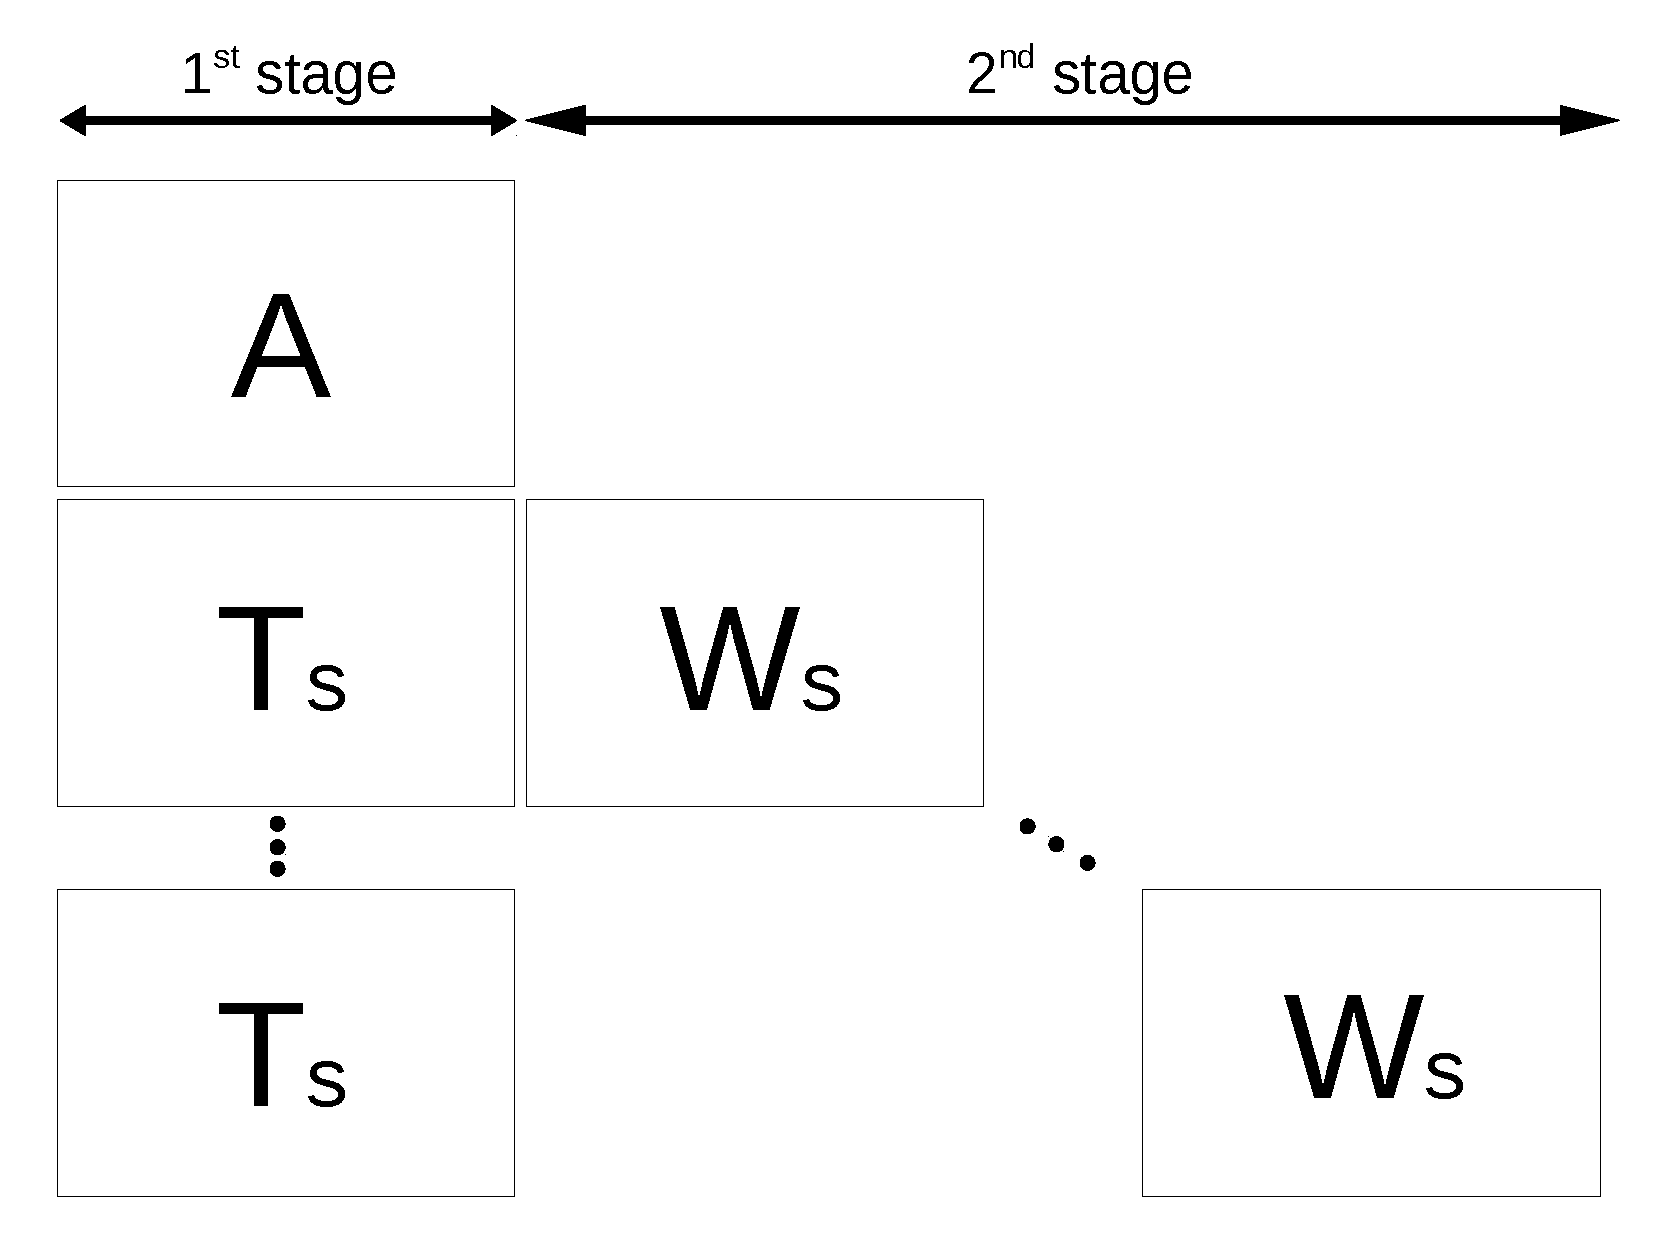
\includegraphics[width=0.7\linewidth]{drawings/stagewise_sparsity}
		\caption{Three independent blocks in SIP}
		\label{fig:stagewise_sparsity}
	\end{figure}

	
	%\kk{This section looks more or less a manual; but, should provide more than that. For example, the section should contain the answers to the questions: Why do we care about this? What kind of information do we want to provide? Does it provide any information for testing algorithms? The manual-like information would better go to the package website (not research paper).}
	%\yoc{The answers to the questions are discussed in Section 3: the reasons why variable types, number of components (size), sparsity are important.}
	
	%\noindent\begin{minipage}{.45\textwidth}
	%\begin{lstlisting}[frame=single,language=julia]
	%type Size
	%	InstanceName::String
	%	nCont1::Int
	%	nBin1::Int
	%	nInt1::Int
	%	nCont2::Int
	%	nBin2::Int
	%	nInt2::Int
	%	nCont::Int
	%	nBin::Int
	%	nInt::Int
	%	nRow::Int
	%	nCol::Int
	%	nNz::Int
	%	Size() = new()
	%end
	%\end{lstlisting}
	%\end{minipage}\hfill
	%\begin{minipage}{.45\textwidth}
	%\begin{lstlisting}[frame=single,language=julia]
	%type Sparsity
	%	InstanceName::String
	%	nRow1::Int
	%	nCol1::Int
	%	nNz1::Int
	%	sparsity1::Float64
	%	nRow2::Int
	%	nCol2::Int
	%	nNz2::Int
	%	sparsity2::Float64
	%	nRowC::Int
	%	nColC::Int
	%	nNzC::Int
	%	sparsityC::Float64
	%	nRow::Int
	%	nCol::Int
	%	nNz::Int
	%	sparsity::Float64
	%	Sparsity() = new()
	%end
	%\end{lstlisting}
	%\end{minipage}
	\pagebreak
	\subsubsection{function \texttt{getSize()}}
	To get the size information of an instance, excute the following function.
	\begin{lstlisting}[frame=single,language=julia]
	function getSize(model::JuMP.Model, INSTANCE_NAME::String="")::Size
	\end{lstlisting}
	The function \texttt{getSize()} takes \jumpmodel-type object as a necessary input argument and returns \texttt{Size}-type object defined as follows.
	\begin{lstlisting}[frame=single,language=julia]
	mutable struct Size
		INSTANCE_NAME::String    # instance name
		nCont1::Int             # number of continuous variables in 1st stage
		nBin1::Int              # number of binary variables in 1st stage
		nInt1::Int              # number of integer variables in 1st stage
		nCont2::Int             # number of continuous variables in 2nd stage    
		nBin2::Int              # number of binary variables in 2nd stage
		nInt2::Int              # number of integer variables in 2nd stage    
		nCont::Int              # number of continuous variables in total      
		nBin::Int               # number of binary variables in total      
		nInt::Int               # number of integer variables in total      
		nRow::Int               # number of rows in coefficient matrix in extensive form
		nCol::Int               # number of columns in coefficient matrix in extensive form
		nNz::Int                # number of nonzero values in coefficient matrix in extensive form
		Size() = new()
	end
	\end{lstlisting}
	
	\subsubsection{function \texttt{getSparsity()}}
	To get the sparsity information of an instance, excute the following function.
	\begin{lstlisting}[frame=single,language=julia]
	function getSparsity(model::JuMP.Model, INSTANCE_NAME::String="")::Sparsity
	\end{lstlisting}
	The function \texttt{getSparsity()} takes \jumpmodel-type object as a necessary input argument and returns \texttt{Sparsity}-type object.
	\begin{lstlisting}[frame=single,language=julia]
	mutable struct Sparsity
		INSTANCE_NAME::String    # instance name
		nRow1::Int              # number of rows in 1st stage-only block (block A)
		nCol1::Int              # number of columns in 1st stage-only block (block A)
		nNz1::Int               # number of nonzero values in 1st stage-only block (block A)
		sparsity1::Float64      # sparsity ([0,1] scale) of 1st stage-only block (block A)
		nRow2::Int              # number of rows in 2nd stage-only block (block W)
		nCol2::Int              # number of columns in 2nd stage-only block (block W)
		nNz2::Int               # number of nonzero values in 2nd stage-only block (block W)
		sparsity2::Float64      # sparsity ([0,1] scale) of 2nd stage-only block (block W)
		nRowC::Int              # number of rows in technology block (block T)
		nColC::Int              # number of columns in technology block (block T)
		nNzC::Int               # number of nonzero values in technology block (block T)  
		sparsityC::Float64      # sparsity ([0,1] scale) of technology block (block T)
		nRow::Int               # number of rows in total
		nCol::Int               # number of columns in total
		nNz::Int                # number of nonzero values in total
		sparsity::Float64       # sparsity ([0,1] scale) in total
		Sparsity() = new()
	end
	\end{lstlisting}
	
	\pagebreak
	\subsubsection{Five functions for plotting sparsity pattern}
	To plot the sparsity patterns of coefficient matrices, we provide the following functions.
	\begin{lstlisting}[frame=single,language=julia]
	function plotConstrMatrix(model::JuMP.Model, INSTANCE_NAME::String="instance", DIR_NAME::String="$(dirname(@__FILE__))/../plot")
	
	function plotFirstStageBlock(model::JuMP.Model, INSTANCE_NAME::String="instance_block_A", DIR_NAME::String="$(dirname(@__FILE__))/../plot")
	
	function plotSecondStageBlock(model::JuMP.Model, INSTANCE_NAME::String="instance_block_W", DIR_NAME::String="$(dirname(@__FILE__))/../plot")
	
	function plotTechnologyBlock(model::JuMP.Model, INSTANCE_NAME::String="instance_block_T", DIR_NAME::String="$(dirname(@__FILE__))/../plot")
	
	function plotAllBlocks(model::JuMP.Model, INSTANCE_NAME::String="instance", DIR_NAME::String="$(dirname(@__FILE__))/../plot")
	
	function plotAll(model::JuMP.Model, INSTANCE_NAME::String="instance", DIR_NAME::String="$(dirname(@__FILE__))/../plot")
	\end{lstlisting}
	All the functions above take up to three input arguments:
	\begin{quote}
		\noindent\underline{\texttt{model}} (necessary, positional) The \jumpmodel-type object of which we want to draw plots.
	\end{quote}
	
	\begin{quote}
		\noindent\underline{\texttt{INSTANCE\_NAME}} (optional, positional) The \texttt{String}-type argument that will be the name of plot files. If not specified, \texttt{INSTANCE\_NAME="instance\_"} as a default. Plots are stored in .pdf format.
	\end{quote}
	
	\begin{quote}
		\noindent\underline{\texttt{DIR\_NAME}} (optional, positional) The \texttt{String}-type argument to indicate a directory where the files are stored. The .pdf file is stored in the default folder ``\texttt{$\sim$/Siplib/plot/}'' unless the argument \texttt{DIR\_NAME} is specified.
	\end{quote}
	The function \texttt{plotConstrMatrix} plots the whole constraint matrix of extensive form. For example, the following command lines plot Fig. \ref{fig:plotall_b}.
	\begin{lstlisting}[frame=single,language=julia]
	params_arr = [2,2,2,2]	                        # declare parameters
	problem = :DCAP	                                # declare problem
	INSTANCE_NAME = getInstanceName(problem, params_arr)	# get instance name
	model = getModel(problem, params_arr)	    # construct JuMP.Model object
	plotConstrMatrix(model, INSTANCE_NAME)               # plot extensive form constraint matrix   
	\end{lstlisting}
	
	The functions \texttt{plotFirstStageBlock()}, \texttt{plotSecondStageBlock()}, and
	 
	 \noindent\texttt{plotTechnologyBlock()} all take \jumpmodel-type object and plots each block. For example, the following command lines plot Fig. \ref{fig:plotall_a}, \ref{fig:plotall_c}, and \ref{fig:plotall_d}.
	\begin{lstlisting}[frame=single,language=julia]
	params_arr = [2,2,2,2]	                        # declare parameters
	problem = :DCAP	                                # declare problem
	INSTANCE_NAME = getInstanceName(problem, params_arr)	# save instance name
	model = getModel(problem, params_arr)	    # construct JuMP.Model object
	plotFirstStageBlock(model, INSTANCE_NAME)               # plot 1st stage block
	plotSecondStageBlock(model, INSTANCE_NAME)               # plot 2nd stage block
	plotTechnologyBlock(model, INSTANCE_NAME)               # plot technology block
	\end{lstlisting}
	
	One might want to draw all the plots at once. The following two functions are defined to do that.
	\begin{lstlisting}[frame=single,language=julia]
	plotAllBlocks(model, INSTANCE_NAME)               # plot all blocks A, W, and T, respectively
	plotAll(model, INSTANCE_NAME)               # plot all the plots above: EF constraint matrix and blocks A, W, T
	\end{lstlisting}
	\begin{figure}[H]
	\centering
	\subfloat[][DCAP\_2\_2\_2\_2\_block\_A.pdf]
	{
		\centering
\includegraphics[width=0.45\linewidth]{DCAP_2_2_2_2_block_A}
		\label{fig:plotall_a}
	}
	~
	\subfloat[][DCAP\_2\_2\_2\_2.pdf]
	{
		\centering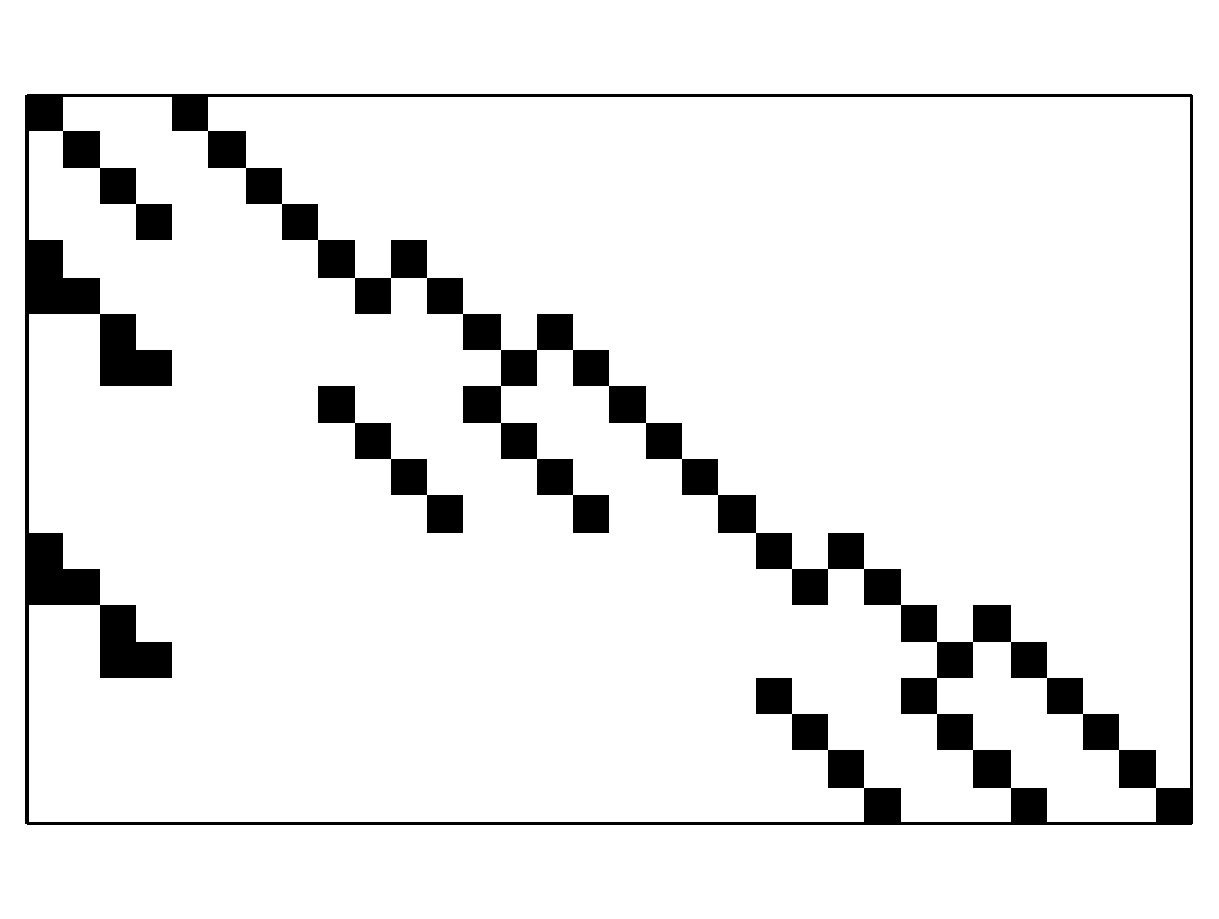
\includegraphics[width=0.45\linewidth]{DCAP_2_2_2_2}
		\label{fig:plotall_b}
	}
	
	\subfloat[][DCAP\_2\_2\_2\_2\_block\_T.pdf]
	{
		\centering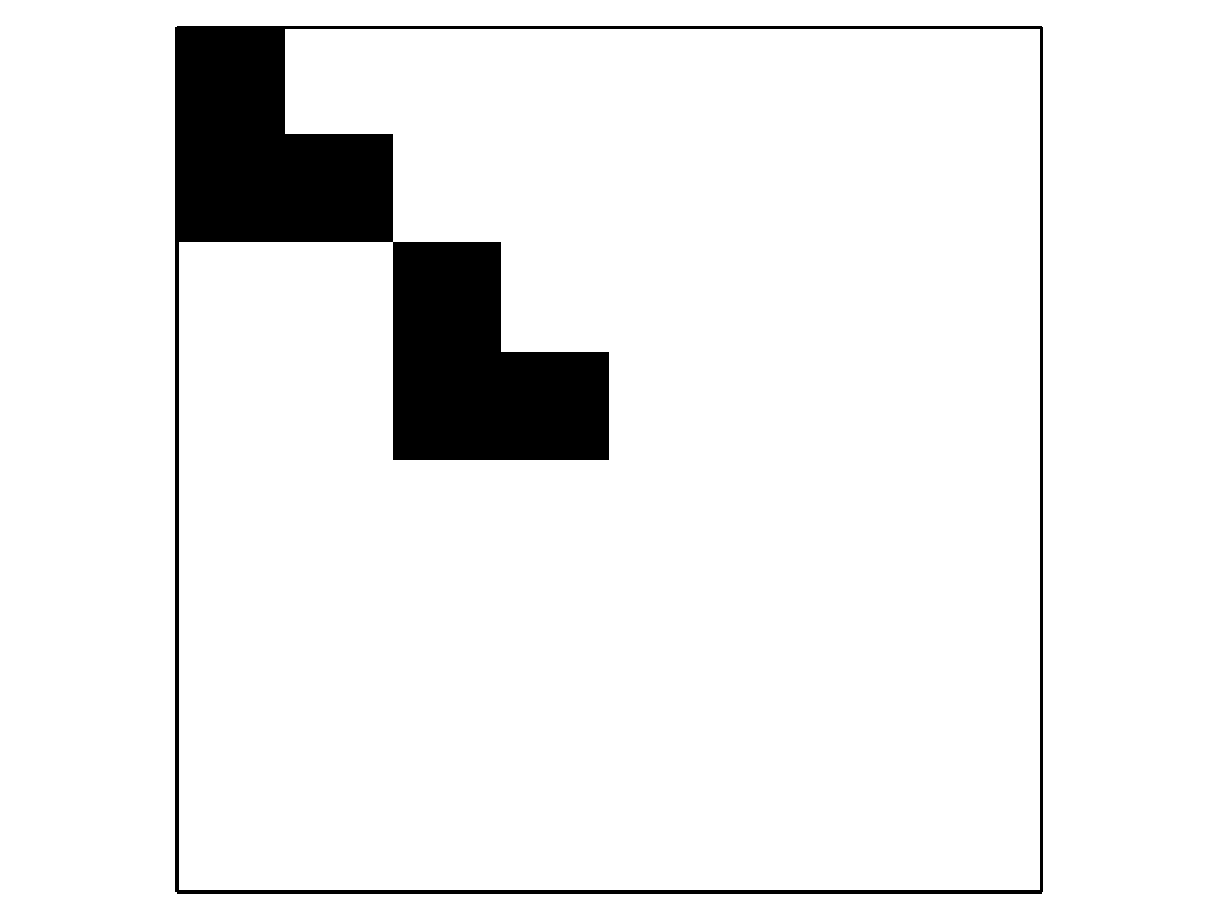
\includegraphics[width=0.45\linewidth]{DCAP_2_2_2_2_block_T}
		\label{fig:plotall_c}
	}
	~
	\subfloat[][DCAP\_2\_2\_2\_2\_block\_W.pdf]
	{
		\centering
\includegraphics[width=0.45\linewidth]{DCAP_2_2_2_2_block_W}
		\label{fig:plotall_d}
	}

	\caption{Plots drawn by executing function \texttt{plotAll}}
%	\begin{minipage}
%	\end{minipage}
	\label{fig:plotall}
\end{figure}
	By executing \texttt{plotAll()}, one can obtain all the plots in Fig. \ref{fig:plotall}.
		
	
	
	\bibliographystyle{spbasic}      % basic style, author-year citations
	%\bibliographystyle{spmpsci}      % mathematics and physical sciences
	%\bibliographystyle{spphys}       % APS-like style for physics
	%\bibliography{}   % name your BibTeX data base
	\begin{thebibliography}{9} 
		\bibitem{web:SIPLIB1}
		S. Ahmed, R. Garcia, N. Kong, L. Ntaimo, G. Parija, F. Qiu, S. Sen. SIPLIB: A Stochastic Integer Programming Test Problem Library. http://www.isye.gatech.edu/~sahmed/siplib, 2015.
		\bibitem{journal:AG2004}
		S. Ahmed and R. Garcia. "Dynamic Capacity Acquisition and Assignment under Uncertainty," Annals of Operations Research, vol.124, pp. 267-283, 2003.
		\bibitem{journal:TPP2017}
		R. Tadei, G. Perboli, and F. Perfetti, The multi-path traveling salesman problem with stochastic travel costs, EURO Journal on Transportation and Logistics, 2017
		\bibitem{journal:JSW1999}
		Soheila Jorjani, Carlton H. Scott, and David L. Woodruff, Selection of an optimal subset of sizes, International Journal of Production Research, 1999	
		\bibitem{journal:AAD2014}
		Gustavo Angulo, Shabbir Ahmed, and Santanu S. Dey, Improving the integer L-shaped method, 2014.
		\bibitem{journal:PO2013}
		Anthony Papavasiliou and Shmuel S. Oren, Multiarea stochastic unit commitment for high wind penetration in a transmission constrained network, Operations Research, 2013
		\bibitem{journal:NS2005}
		Lewis Ntaimo and Suvrajeet Sen, The million-variable ``March'' for stochastic combinatorial optimization, Journal of Global Optimization, 2005
	\end{thebibliography}
	
\end{document}
